\subsection{Concentrated Placement and Startup Under Load}
\label{sec:mumbai-startup}

We conducted a separate Oracle Cloud cluster experiment with an isolated subscriber
Deployment and Service to examine what happens when persistent TCP connections remain on one Pod. In an initial 4,000-subscription static calibration, ten delivery
connections and two probes terminated on one Pod. Adding three Ready Pods did
not relocate these sockets: the source retained all twelve established
connections, while each added Pod had none. The clients nevertheless received
and acknowledged events while subscription activation was still progressing.
Full activation took approximately 1,398.4 seconds; the completed run reconciled
137,008 observed deliveries with confirmed ACKs. This shows the difference between having server capacity and reaching it
through existing persistent connections.

A later frozen-DQL test used 2,000 other subscriptions, divided
equally among four event-type groups. One client attached five connections,
each carrying 400 subscriptions, to the single source Pod. Three destination
Pods became Ready before standby bindings were activated. The client used
32 processing workers without an artificial processing delay, ten message
permits per subscription, and a window of 32 outstanding activation requests.
Exact lifecycle records used batched SQLite transactions with FULL
synchronization and a mandatory flush at measurement and closure boundaries.
The earlier calibration used a different subscription population and recorder
settings. The two timing records are therefore reported as separate
experiments rather than a matched static-policy comparison.

\begin{table}[!htbp]
  \caption{Measured isolated Oracle Cloud cluster connection-rebalancing qualification.
  These values describe one live run, distinct from the earlier
  20,000-subscription deployment.}
  \Description{Four available Pods, two thousand subscriptions, five active
  connections, three migrations of four hundred subscriptions, and exact
  reconciliation of seventy-three thousand six hundred thirty-nine observed
  deliveries. The source population falls from two thousand to eight hundred.}
  \label{tab:mumbai-isolated-recovery}
  \centering
  \small
  \begin{tabular}{p{0.65\linewidth}r}
    \toprule
    Measurement & Observed value \\
    \midrule
    Available Pods / subscribed Pods before and after & 4 / 1 and 3 \\
    Subscriptions / active connections / probe & 2,000 / 5 / 1 \\
    Time to 50\% / 90\% / full activation (s) & 238.066 / 388.139 / 426.305 \\
    Committed connection migrations / subscriptions moved & 3 / 1,200 \\
    Source subscriptions before / after & 2,000 / 800 \\
    Final subscribed-Pod populations & 800, 800, 400 \\
    Handoff times, in execution order (s) & 10.878, 10.992, 10.648 \\
    Source-drain waits, in execution order (s) & 6.069, 6.174, 6.848 \\
    Delivered / processed / receipt-confirmed ACKs & 73,639 / 73,639 / 73,639 \\
    Unresolved observed attempts at closure & 0 \\
    Recorded ACK failures / duplicate candidates & 0 / 0 \\
    \bottomrule
  \end{tabular}
\end{table}

The frozen controller committed three complete connection replacements,
each moving 400 subscriptions through a retained probe. The source population
fell from 2,000 to 800, a reduction of
$(2{,}000-800)/2{,}000=60\%$. Two destination Pods acquired 400 and 800
subscriptions. The active-connection count remained five, and all 2,000
subscriptions were confirmed in the final topology after the two-minute hold.
The migrations therefore changed which Pods served these subscriptions
without increasing the client's active-connection count.

\begin{figure}[!htbp]
  \centering
  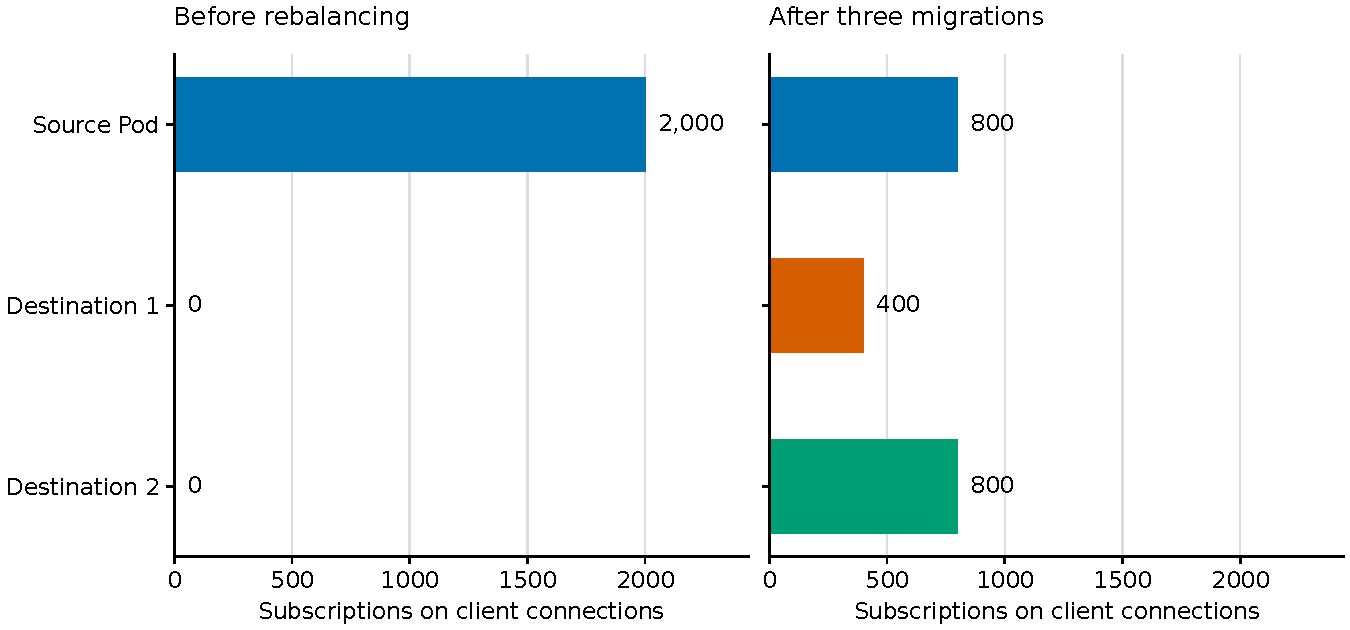
\includegraphics[width=\textwidth]{figures/observed-pod-redistribution.pdf}
  \caption{Verified client subscription placement before and after three
  frozen-DQL connection migrations in the Oracle Cloud cluster. Bars aggregate the client's
  receipt-confirmed bindings by serving Pod. Initial zeros mean no bindings
  belonging to this client, not a measurement of every cluster subscription.
  Both panels account for the same 2,000 subscriptions and five connections.}
  \Description{The initial source has two thousand subscriptions. After
  rebalancing it has eight hundred; two destinations have four hundred and
  eight hundred. No subscription is removed from the population.}
  \label{fig:mumbai-isolated-placement}
\end{figure}
\FloatBarrier

Figure~\ref{fig:mumbai-isolated-placement} shows the main operational effect:
newly available capacity becomes reachable by moving subscription-bearing
connections. It reports verified connection endpoints, rather than estimating changes
between observations. A probe was first resampled because it did not
offer an admissible improvement. Eleven later decision intervals selected
stay while backlog telemetry was incomplete; migration resumed when the
observation checks passed. The online and target network parameters remained
identical to the loaded checkpoint, while valid transitions were retained.

\subsubsection{Activation and Delivery Coexistence}

For subscription $k$, let $t_k^{\mathrm{send}}$ be activation submission time and $t_k^{\mathrm{ready}}$ its
successful receipt time, relative to the start of activation. At elapsed
time $s$ in seconds, the cumulative completion count is
$A^{\mathrm{act}}(s)=\sum_{k=1}^{2000}\mathbf{1}\{t_k^{\mathrm{ready}}\leq s\}$,
and $2000-A^{\mathrm{act}}(s)$ is the pending count. This separates attachment from
confirmed activation and makes startup delay visible even while events flow.
The 50th, 90th and 100th completion percentiles were 238.066, 388.139 and
426.305 seconds, respectively. No activation retry was needed in this run.

\begin{figure}[!htbp]
  \centering
  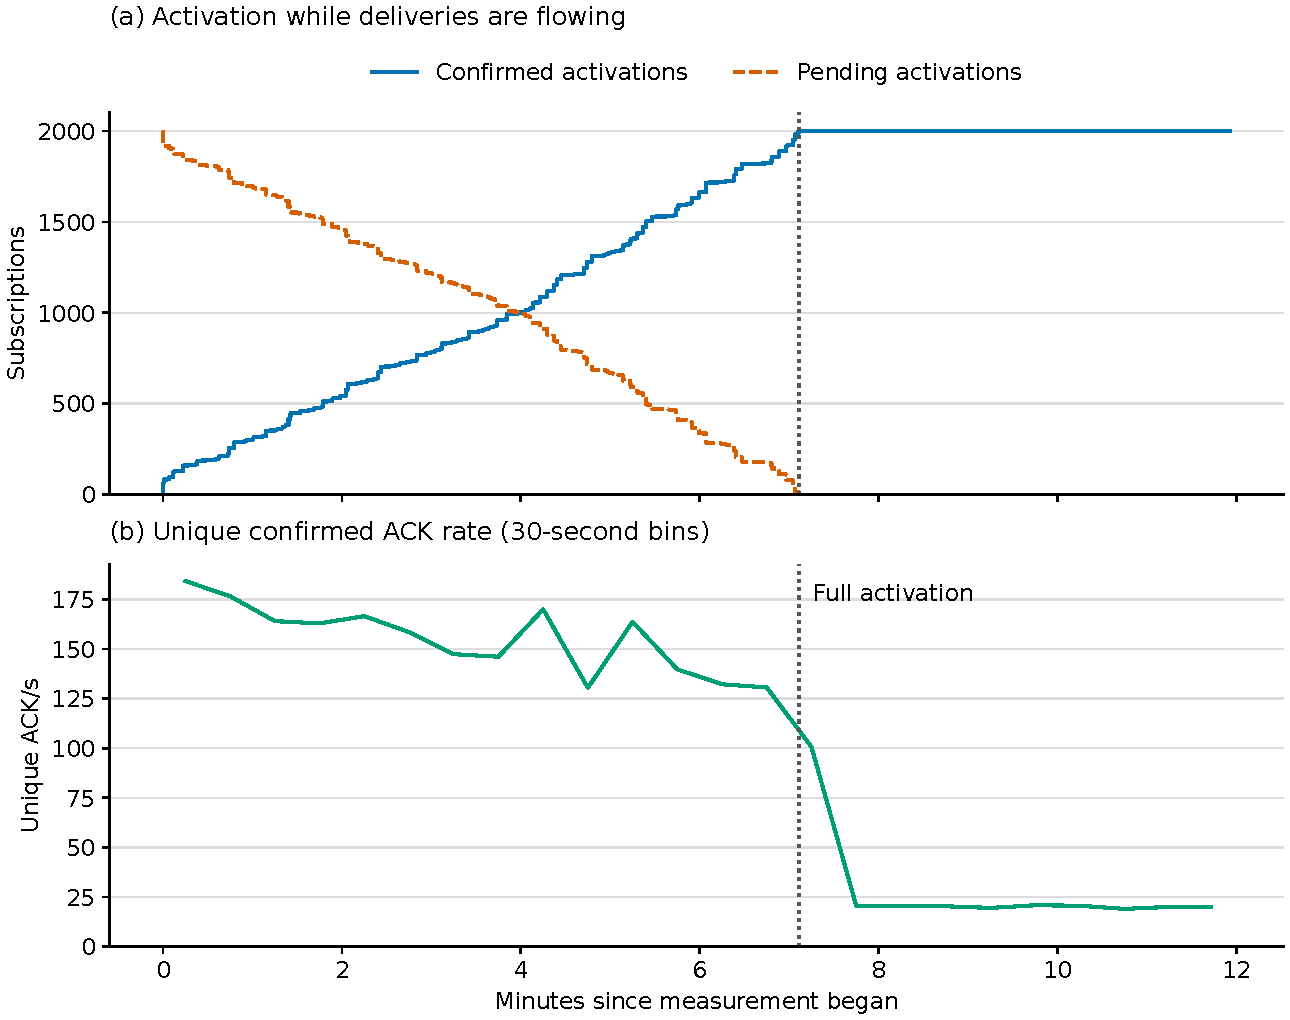
\includegraphics[width=0.94\textwidth]{figures/activation-and-ack-rate.pdf}
  \caption{Activation and acknowledged delivery in the isolated Oracle Cloud cluster run.
  Top: confirmed and pending activation counts. Bottom: distinct observed
  subscription--message pairs whose first successful ACK receipt occurs in
  each 30-second bin, divided by that bin's actual duration. The dotted line
  marks full activation. DQL decisions start after this line.}
  \Description{Activation rises to two thousand while pending activations
  fall to zero. ACKs arrive throughout startup. The later delivery rate falls
  as the consumed workload changes; the curve is not a matched throughput
  comparison with a static policy.}
  \label{fig:mumbai-live-activation}
\end{figure}
\FloatBarrier

Figure~\ref{fig:mumbai-live-activation} retains the startup interval rather
than treating it as discarded warm-up. Of 73,587 distinct first ACKs inside
the 716.017-second measurement window, 66,400 occurred before full activation.
A further 52 attempts completed during shutdown, bringing final reconciled
deliveries to 73,639. The rate curve describes consumption of existing queued
work. It describes startup and workload drainage rather than constant-offered-load
capacity. DQL begins after full activation, so these measurements establish
delivery during startup followed by redistribution. Activation time precedes
the policy intervention.

\begin{figure}[!htbp]
  \centering
  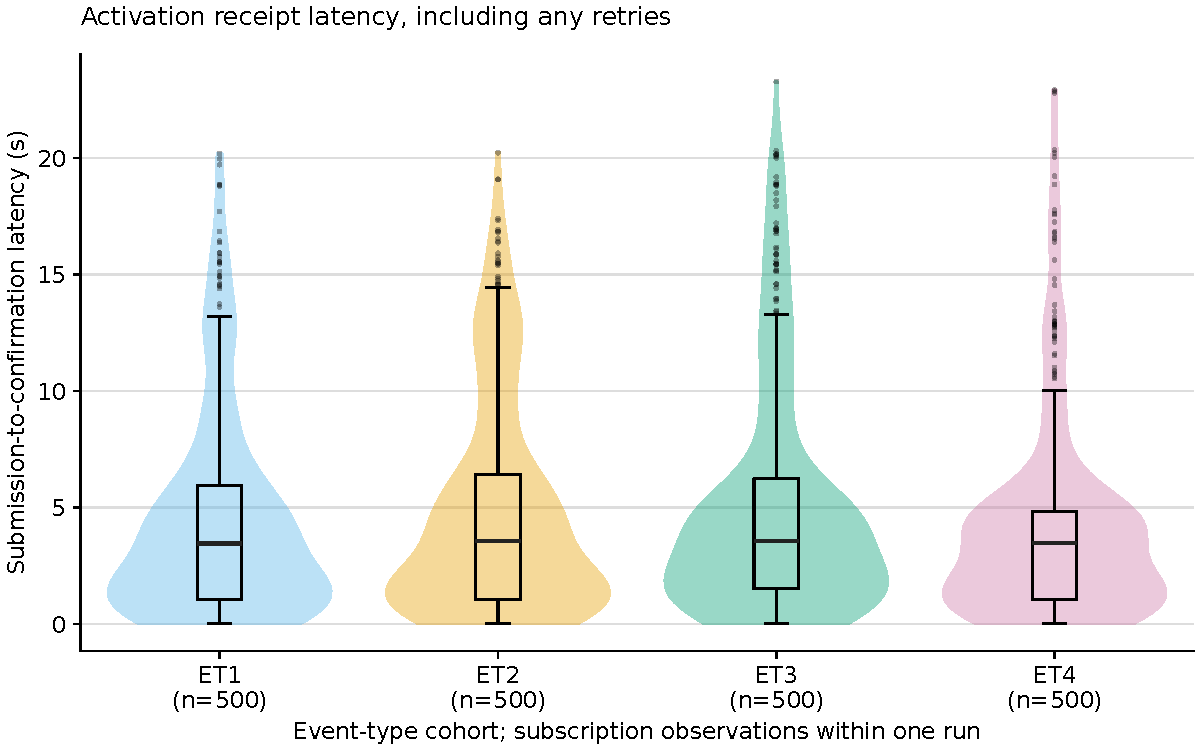
\includegraphics[width=0.92\textwidth]{figures/activation-latency-violin-box.pdf}
  \caption{Within-run activation latency $\ell_k^{\mathrm{act}}=t_k^{\mathrm{ready}}-t_k^{\mathrm{send}}$ for 500 subscriptions
  in each event-type cohort. Violin widths show smoothed empirical density;
  boxes show the interquartile range and median. Whiskers use 1.5 interquartile
  ranges, with observations beyond them retained as points. These are
  subscription observations in one run, not independent cluster trials.}
  \Description{Four violin and box plots show activation receipt latencies.
  Medians are approximately three and a half seconds, with observed upper
  tails reaching roughly twenty to twenty-three seconds.}
  \label{fig:mumbai-activation-latency}
\end{figure}
\FloatBarrier

Figure~\ref{fig:mumbai-activation-latency} distinguishes an individual request's
latency from the time to activate the complete population. Cohort medians were
3.443, 3.560, 3.567 and 3.476 seconds; nearest-rank 99th percentiles were
18.805, 16.907, 20.072 and 20.038 seconds. The subscriptions share upstream services and scheduling conditions, so their
observations are dependent. The distributions describe within-run variation,
without estimating a between-policy confidence interval. A concurrent
thread snapshot found fourteen subscription handlers waiting for upstream
transition confirmation. This locates the observed startup bottleneck in
upstream confirmation waits; the snapshot does not establish CPU saturation.

The complete ledger covers observed delivery attempts, with publisher-to-Queue
event counts outside its scope. This qualification establishes
receipt-confirmed activation under delivery load, probe-based redistribution
with a 60\% reduction in source subscriptions, and reconciled closure. The
recorded delivery rates include workload depletion and startup, so the
experiment reports redistribution rather than an isolated throughput effect.
